\documentclass[]{ifacconf}  % Comment this line out
                                                          % if you need a4paper

\usepackage{graphicx}      % include this line if your document contains figures
\usepackage{natbib}        % required for bibliography. Does not work with ifac format together with hyperref package
%\usepackage{hyperref}
\usepackage{subfigure}
\usepackage{amsfonts}
\usepackage{amsmath}
\usepackage{amssymb}
\usepackage{makeidx}
\usepackage{epsfig}
%\usepackage{color}
%\usepackage[dvips]{color}
%\usepackage{amsthm}
\usepackage{makeidx,epsfig}
\usepackage{multirow}
\usepackage{mathrsfs}
%\usepackage[T1]{fontenc}          %%%%%% INSERIRE PER ACCENTO!!!!!!!!!!!!
%\usepackage[utf8]{inputenc}
%\usepackage[italian]{babel}
%\usepackage[table]{xcolor}
\usepackage{todonotes}
%\usepackage{menukeys}
\usepackage{algorithm,algpseudocode}
\usepackage{accents}
\usepackage{booktabs}

% balance last page
\usepackage{flushend}

%\usepackage[font=small,justification=raggedright]{caption}
\newcommand\munderbar[1]{%
	\underaccent{\bar}{#1}}




\newcommand\todoin[2][]{\todo[inline, caption={2do}, #1]{
		\begin{minipage}{\textwidth-4pt}#2\end{minipage}}}
%\hypersetup{citecolor=black, colorlinks=false, linkcolor=black, pdfborder={0 0 0}}
\providecommand{\ad[1]}{{\color{blue}#1}}

%
%%===============================================================================
%
%\newtheorem{algorithm}{Algorithm}
%\newtheorem{assumption}{Assumption}
\newtheorem{theorem}{Theorem}
\newtheorem{corollary}[theorem]{Corollary}
\newtheorem{definition}{Definition}
\newtheorem{example}{Example}
\newtheorem{lemma}[theorem]{Lemma}
\newtheorem{proposition}[theorem]{Proposition}
\newtheorem{problem}{Problem}
\newtheorem{remark}{Remark}
\newtheorem{assumption}{Assumption}


%==============================================================================================================
%==============================================================================================================

\begin{document}

\begin{frontmatter}
	
	\title{Data-driven Switched Affine Modeling for Model Predictive Control\thanksref{footnoteinfo}} 
	% Title, preferably not more than 10 words.
	
	\thanks[footnoteinfo]{This work was supported by project \emph{INnovating City Planning through Information and Communication Technologies} (INCIPICT), and by TerraSwarm, one of six centers of STARnet, a Semiconductor Research Corporation program sponsored by MARCO and DARPA, and by the Italian Government under Cipe resolution n.135 (Dec. 21, 2012).}
	
	\author[First,Second]{Francesco Smarra} 
	\author[Second]{Achin Jain} 
	\author[Second]{Rahul Mangharam}
	\author[First]{Alessandro D'Innocenzo}
	
	\address[First]{Department of Information Engineering, Computer Science and Mathematics, University of L'Aquila, Via Vetoio, 67100 L'Aquila, Italy \\(e-mail: [francesco.smarra,alessandro.dinnocenzo]@univaq.it).}
	\address[Second]{Department of Electrical and Systems Engineering, University of Pennsylvania, 200 South 33rd Street, 19104 Philadelphia, PA, USA (e-mail: [fsmarra,achinj,rahulm]@seas.upenn.edu)}

\begin{abstract}
Model Predictive Control (MPC) is a well consolidated technique to design optimal control strategies, leveraging the capability of a mathematical model to predict the system's behavior over a predictive horizon. 
However, building physics-based models for large scale systems, such as buildings and process control, can be cost and time prohibitive.
To overcome this problem we propose in this paper a methodology to exploit machine learning techniques (i.e. regression trees and random forests) in order to build a state-space switched affine dynamical model of a large scale system only using historical data.
Finite Receding Horizon Control (RHC) setup using control-oriented data-driven models based on regression trees and random forests is presented as well.
A comparison with an optimal MPC benchmark and a related methodology is provided on an energy management system to show the performance of the proposed modeling framework.
Simulation results show that the proposed approach is very close to the optimum and provides better performance with respect to the related methodology in terms of cost function optimization.
\end{abstract}

\begin{keyword}
	Data-driven modeling, data-driven model predictive control, machine learning, switched systems.
\end{keyword}

\end{frontmatter}
%==============================================================================================================
%==============================================================================================================

\section{INTRODUCTION}\label{secIntro}
Model Predictive Control (MPC) is a well known control strategy used to design optimal control actions to optimize desired system performance while guaranteeing a desired system behavior.
To provide such an optimal control strategy, MPC uses mathematical models to predict system behavior over a horizon.
MPC has been widely applied in past years to control a large variety of systems, as for example energy systems such as smart buildings, smart grids and power systems \cite{MaTCST2015,OldewurtelEB2012,MaasoumyEB2014,IovineIFAC2017,WrightTCST2008,LiuTII2013}.
However, creating a physics-based models for large-scale systems, as the ones mentioned above, can be cost and time prohibitive \cite{SturzeneggerTCST2016,ZacekovaAE2014}.
To overcome this issue, a possibility is to use machine learning algorithms to create models using only historical data available to the system.
Several works, \cite{Macarulla2017,Afram2017,Ferreira2012} and others, deal with this problem and use machine learning algorithms to construct data-driven models to be used for control.
Nevertheless, none of these works addressed the problem of creating data-driven state models only using data, that could be used to predict the state evolution over a horizon in an MPC problem formulation.
To the best of authors' knowledge, such problem has been addressed for the first time in \cite{BehlAE2016}, where data-driven models, built using regression trees-based algorithms, have been developed to enable one-step lookahead closed-loop predictive control for the demand-response problem in buildings.
This approach has been extended in \cite{JainCDC2017}, where the authors proposed a regression trees and random forests-based Data Predictive Control (DPC) strategy, that implements finite Receding Horizon Control (RHC) over an horizon of arbitrary length.
However, both the aforementioned approaches make use of data-driven \emph{static} models, where the input-output relation is represented by affine functions.
As a consequence, such modeling framework does not take into account the presence of an internal state evolution and loose the information, over the prediction horizon, of the past inputs applied to the system. 
This translate in a lack of internal consistency of the model and in a loss of control performance, as we will show in the simulations. 
Furthermore, due to the lack of an internal state, system's properties, such as stability, structural properties, etc., cannot be studied.

\emph{\textbf{Main Contribution.}} The goal of this paper is to provide a new methodology to create a state-space switched affine dynamical model of a system using only historical data, leveraging regression trees and random forests, and without any knowledge about its physics-based modeling. We then use this model to setup an MPC problem to optimally control the system's behavior.
The idea is to bridge machine learning and control to build control-oriented models that can be used to provide system guarantees.
This modeling technique has the advantage to keep the simplicity of the model identification methodology used to create data-driven models for DPC, while guaranteeing the presence of an internal state typical of state-space models.
This is useful when one has to model complicated large-scale systems, where system dynamics interact in a complicated way, and hence obtaining a physics-based mathematical formulation can be prohibitive.
More precisely, we derive a Switched Affine (SA) data-driven model using regression trees and random forests algorithms.
One of the main reasons for choosing regression trees resides in the fact that, other than providing good model accuracy, they are by design highly interpretable, which is a fundamental desirable quality in any model. We then use this technique to setup an MPC problem both for the model obtained using Regression Trees (SAMPC-RT) and for the model obtained using Random Forests (SAMPC-RF). 
To show the validity of our approach, we compare our methodology with DPC using a bilinear model of a building with $12$ states, $4$ inputs and $8$ disturbances, whose parameters were identified using experiments on a building in Switzerland (\cite{OldewurtelPHD2011}).
As an optimal reference to compare our approach to, we consider a benchmark MPC controller with perfect knowledge of the model.
We show that the proposed approach outperform DPC in terms of cost function minimization, providing results that are closer to the optimum.
Although we said this approach fits well for large-scale systems, where obtaining a mathematical model can be prohibitive, we specifically consider in this paper the aforementioned model, which we have a formulation of, otherwise a comparison with the optimal solution would not be possible.
This contribution is a further step towards bridging machine learning, more precisely regression trees and random forests, with control theory, and in particular predictive control.
The application to more complex systems is part of our future work.
\begin{remark}
	Although in this work we do not provide analysis or guarantees of system's properties, as we criticized for DPC, there are many results in literature to investigate them for switched systems (not necessarily for MPC), as for example \cite{MullerJPC2012,BraatzAutomatica2016,DanielsonACC2016,HespanhaTAC2004,LiberzonAutomatica1999,WangTAC2002,LeeAutomatica2002}, and many others. The methodology we propose can also be used to build Piece-Wise Affine models that can be controlled using, for example, the hybrid MPC techniques proposed in \cite{LazarTAC2006,BemporadAutomatica1999}. However,
	combine these works with our approach is out of the scope of this paper and it is venue for future research.
\end{remark}

\emph{\textbf{Paper organization.}} In Section \ref{secDPC} we briefly recall the DPC formulation. In Section \ref{secDataDrivenModeling}, as the main contribution of this paper, we present a new methodology to derive, starting from a set of data, switched affine models to capture system's dynamics, and setup a Model Predictive Control problem that uses such data-driven model.
In Section \ref{secCaseStudy} we provide a comparison of the proposed methodology to DPC and to the MPC benchmark in a building automation case study.

\textbf{\emph{Notation.}} We denote by $I$ and $\bold{0}$ respectively the identity matrix and a matrix with all the entries equal to $0$ of appropriate dimensions, by $det(A)$ the determinant of matrix $A$, by $\biguplus$ the disjoint union, and by $|S|$ the cardinality of the set $S$.

\section{Data Predictive Control}\label{secDPC}
In this section we briefly recall first the concept of regression trees partitioning, and then the concept of DPC provided in \cite{JainCDC2017}. 
This will be useful to both better understand and compare the approach we want to propose.
The main idea is to create system models using machine learning algorithms (in the specific case, regression trees and random forests) starting from data, that can be used in a receding horizon control scheme.
Let a dataset $(\mathcal{X},\mathcal{Y})$, where $\mathcal{X} = \{s^x_1,\ldots,s^x_{|\mathcal{X}|}\}$ is the set of predictor variables (or features) samples and $\mathcal{Y} = \{s^y_1 ,\ldots,s^y_{|\mathcal{X}|}\}$ is the set of response variables (system outputs) samples, be given.
Each sample in the dataset corresponds to a measurement over time of system's variables.
The regression trees algorithm creates a tree structure $\mathcal{T}$ by partitioning the set $\mathcal{X}$ into smaller regions, the \emph{leaves} of the tree, following specific rules \cite{Breiman1984classification}.
Each leaf $i$ contains a certain number of samples from $\mathcal{X}$.
In particular, let $\ell_{i} \subset \mathcal{X}$, with $i=1,\ldots,p$, be the set of predictor variable samples contained in the $i^{th}$ leaf of $\mathcal{T}$. The leaves of $\mathcal{T}$ form a partition of $\mathcal{X}$:
\small
\begin{align}\label{distSetPartition}
\mathcal{X}=\biguplus_{i=1}^{p}{\ell_{i}}, \quad \left(\ell_{\alpha}\cap \ell_{\beta}=\varnothing,\,\forall \alpha\neq \beta \right).
\end{align}
\normalsize
Then, the algorithm associates to each leaf $\ell_i$ a prediction $\hat{y}_i$ as the average of the response values associated to each sample in $\ell_i$. 
This algorithm is known as CART (see \cite{Breiman1984classification} for more details). 
However, since the prediction provided by the tree is an averaged value, the learning procedure described above needs to be modified to be applied in a RHC problem setup.
To this aim, the following approach has been addressed in \cite{JainCDC2017}.

Let us consider $\mathcal{X}$ as the set containing control inputs $u\in\mathbb{R}^m$, disturbances $d\in\mathbb{R}^r$ and state variables $x\in\mathbb{R}^n$, and $\mathcal{Y}$ as the set containing the output variable $y\in\mathbb{R}$. Without any loss of generality and for the sake of simplicity, we consider only a single output, but the discussion can be generalized considering different trees for different outputs, as we show in this paper, or multi-output trees, as shown in \cite{JainTCPS2017}.
Each sample in the dataset is a vector containing the measured values of the variables at instant $k$.
The set $\mathcal{X}=\{\mathcal{X}_c,\mathcal{X}_d\}$ is partitioned into set $\mathcal{X}_c = \{s_1^c,\ldots,s_{|\mathcal{X}|}^c\}$, of data associated to the $m$ control variables, i.e. $s_k^c = [u_1(k),\ldots,u_m(k)]$, and set $\mathcal{X}_d = \{s_1^d,\ldots,s_{|\mathcal{X}|}^d\}$, of data associated to the $r+n$ disturbance and state variables, i.e. $s_k^d = [d_1(k),\ldots,d_r(k),x_1(k),\ldots,x_n(k)]$.
For $\mathcal{Y} = \{s_1^y,\ldots,s_{|\mathcal{X}|}^y\}$, we have $s_k^y = y(k)$.
The training process to grow a tree $\mathcal{T}$ is divided in 2 steps:
\begin{enumerate}
\item the tree is trained only using $\mathcal{X}_d$, instead of $\mathcal{X}$. 
It is important to note that besides external disturbances, $\mathcal{X}_d$ can also contain past terms of the output $\mathcal{Y}$;
\item affine function models are fit only as a function of variables in $\mathcal{X}_c$ for each leaf $\ell_i$, i.e. only using samples $s_k^c,s_k^y\in\ell_i$, as we will show in Equation \eqref{eqAffineModel}.
\end{enumerate}
This process is illustrated in the left side of Figure \ref{figSeparationVariables}. 
The same methodology can be applied to Random Forests.
The basic idea of the random forests algorithm (\cite{Breiman2001}) is to grow multiple trees, indeed a forest, considering different random subsets of the dataset to train each tree.
The prediction is given by averaging the response of all the trees in the forest, \cite{Breiman2001}.
This reduces the overall variance in the prediction and mitigate the effect of the overfitting.
The price to pay for the identification accuracy improvement is an increase in the computational complexity.
In this paper both approaches are considered.


To obtain a model that can be used in a RHC problem with predictive horizon of arbitrary length $N$, this procedure is used to grow multiple trees $\mathcal{T}_1,\ldots,\mathcal{T}_N$.
Each tree $\mathcal{T}_j$ is used to predict system's response at the $j^{th}$ step of the horizon.
We will discuss this more in detail in the following sections for both Regression Trees and Random Forests.
%Let $\ell_{i_j} = \{s_1,\ldots,s_\epsilon\}$, $i_j=1,\ldots,p_j$, be the $i_j^{th}$ leaf of $\mathcal{T}_j,\ j = 1,\ldots,N$, containing samples $s_1,\ldots,s_\epsilon \in \mathcal{X}_d$. Then the leaves of $\mathcal{T}_j$ form a partition of $\mathcal{X}_d$:
%
%\begin{align}\label{distSetPartition}
%	\mathcal{X}_d=\biguplus_{i_j=1}^{p_j}{\ell_{i_j}}, \quad \left(\ell_{\alpha}\cap \ell_{\beta}=\varnothing,\,\forall \alpha\neq \beta \right).
%\end{align}

\subsection{DPC-RT: DPC with Regression Trees}
Without any loss of generality, and for the sake of simplicity, we consider $n=1$, but the results can be extended to multiple responses considering multiple trees.
The idea is to predict output $y$ over an horizon of length $N$ given the state measurement and the disturbance forecast at the current step. 
Applying the methodology illustrated above, it is possible to build $N$ regression trees $\mathcal{T}_j,\ j=1,\ldots,N$, and associate to each leaf $i_j$ of each tree the following affine static model:
\small
\begin{equation}\label{eqAffineModel}
	y(k+j) = \beta_{i_j}[1\ u(k) \cdots u(k+j)]^\top,\ \forall i_j,\,\forall j,
\end{equation}
\normalsize
where $\beta_{i_j}\in\mathbb{R}^{jm+1}$ is obtained by fitting data in the leaf.
Once these models are created, given the current state measurement and the prediction of the disturbance, i.e. the values of the variables in $\mathcal{X}_d$, in run-time, at each instant $k$, we can narrow down to a leaf of each tree $\mathcal{T}_j$ to find coefficients $\beta_{i_j}$, for $j=1,\ldots,N$, to obtain the linear model \eqref{eqAffineModel} for each step of the horizon (see Algorithm $1$ in \cite{JainCDC2017} for details). This is used to solve the following RHC problem
\begin{problem}\label{pbDPC}
\small
\begin{equation*}
\begin{aligned}
& \underset{u_k}{\text{minimize}} & &  \sum_{j=0}^{N} y_{k+j}^2 Q + u^\top_{k+j} R u_{k+j} +  \lambda\varepsilon_j  \\
& \text{subject to }            & &  y_{k+j}        =   \beta_{i_j} [1\ u_{k} \cdots u_{k+j} ]^\top                   \\
&                               & &  u_{k+j}     \in  \mathcal{U}                                                     \\
&                               & &  |y_{k+j}|     \leq \bar{y} + \varepsilon_j 										\\
&                               & &  \varepsilon_j \geq  0																\\
&                               & &  j              =    0,\ldots,N,            									    \\
\end{aligned}
\end{equation*}
\normalsize
\end{problem}
where slack variables $\varepsilon_j$ ensure recursive feasibility of the algorithm. This problem is solved as in classical MPC. At each time step the optimal $u^*_k,\ldots,u^*_{k+N}$ are computed and only the first one is applied as control input, i.e. $u(k) = u^*_k$.
\begin{figure}[t!]
	\begin{center}
		\includegraphics[width=21pc]{figures/dpc-sepvars.eps}
		\caption{Separation of variables. \textit{Step 1:} Tree $\mathcal{T}_1$ is trained only on the disturbances $\mathcal{X}_d$ as the features. Tree $\mathcal{T}_2$ uses both the disturbances $\mathcal{X}_d$ and the control variables $\mathcal{X}_c$ for splitting and is thus not computationally suitable for control. \textit{Step 2:} In the leaf $\ell_{i_j}$ of trees $\mathcal{T}_j$, a linear regression model parametrized by $\beta_{i_j}$ is defined as a function only of the control variables.}\label{figSeparationVariables}
	\end{center}
\end{figure}

\begin{remark}
	If we did not consider the splitting procedure of the dataset, and we also used input variables to learn the trees, as in the right side of Figure \ref{figSeparationVariables}, the resulting model would not have been suitable for control. This is because, since $u$ is the variable we want to optimize, we do not know its value a priori to go through the trees and determine the correct leaves to find the models to use in the  RHC problem.
\end{remark}

\subsection{DPC-RF: DPC with Random Forests}\label{ssecDPC-RF}
The goal in DPC-RF is to replace model \eqref{eqAffineModel} in Problem \ref{pbDPC} with the following model obtained using Random Forests:
\small
\begin{equation}\label{eqAffineModelRF}
y(k+j) = \Theta_{i_j}[1\ u(k) \cdots u(k+j)]^\top,\ \forall i_j,\,\forall j,
\end{equation}
\normalsize
where $\Theta_{i_j}\in\mathbb{R}^{jm+1}$ is obtained by simply averaging out all the coefficients from all the trees in the forest $j$. 
Both DPC-RT and DPC-RF will be used in Section \ref{secCaseStudy} to compare the methodology we propose in the next section.

%==============================================================================================================
%==============================================================================================================

\section{DATA-DRIVEN SWITCHED AFFINE MODEL}\label{secDataDrivenModeling}
The DPC modeling framework, although simple, is characterized by three main drawbacks:
\begin{enumerate}
\item the models in the leaves are affine functions that provide input-output \emph{static} relations as described in \eqref{eqAffineModel};
\item the current state of the system is not considered by the model equation to predict the system's evolution;
\item to obtain a good prediction accuracy, parameters $\beta_{i_j}$ are different for each step of the horizon.
Therefore in Problem \ref{pbDPC}, the system's evolution at each step does not consider the effect of previously applied inputs.
\end{enumerate}
Basically, in the DPC, system modeling does not take into account an internal state evolution, which is a fundamental characteristic in control systems theory.
The scope of this section is to address this issue providing a data-driven state-space modeling framework using regression trees and random forests.
To this aim we leverage the concept introduced in Section \ref{secDPC}, i.e. splitting the training set, and replace the affine static models \eqref{eqAffineModel} in the leaves with LTI models, obtaining the following switched affine system
\small
\begin{equation}\label{eqSwitchedSystemOriginal}
x(k+1) = A_{\sigma_k}x(k) + B_{\sigma_k}u(k) + f_{\sigma_k},
\end{equation}
\normalsize
\noindent where $\sigma_k: \mathbb{N} \rightarrow \{i_1,\ldots,i_N\}$ is an exogenous signal, that depends on measured values of variables in $\mathcal{X}_d$, and drives the switching rule among the leaves.
We will see in Section \ref{ssecSAMPC-RT} that this task is not trivial, since replacing the affine functions in \eqref{eqAffineModel} with LTI models is not enough to guarantee an internal state evolution, so we propose an extension of the state-space to overcome this problem.
More precisely, the rest of this section is organized in 3 steps:
\begin{enumerate}
	\item in Section \ref{ssecEstimation} we derive, for each leaf of each tree, a model that models the prediction $y(k+j)$ as an affine function of the internal state at time $k$ and of the inputs at time $k,\ldots,k+j$, using regression trees;
	\item in Section \ref{ssecSAMPC-RT} we derive, from the model above, an equivalent switched affine system as in \eqref{eqSwitchedSystemOriginal}, and setup an MPC problem that will be used in Section \ref{secCaseStudy} to show the performance of the proposed approach with respect to DPC and to the optimal MPC benchmark.
	\item in Section \ref{ssecSAMPC-RF} we extend the results obtained in Section \ref{ssecSAMPC-RT} to the case where matrices of \eqref{eqSwitchedSystemOriginal} are estimated using random forests.
\end{enumerate}
In this paper we consider the prediction of the state at next steps as the response variable with its regression terms, i.e. $x(k+j+1) = [y(k+j), y(k+j-1), \ldots, y(k+j-\nu)]^\top$.

\subsection{Model generation}\label{ssecEstimation}
Let us consider a prediction horizon equal to $N$. 
We create $N$ trees $\mathcal{T}_j$, $j = 1,\ldots,N$, each one built using disturbance $d(k+\psi-\delta_d),\ldots,d(k + \psi)$, $\psi\leq j$, and the current state with regression terms $y(k-1),\ldots,x(k-1-\delta_y)$ data from $\mathcal{X}_d$.
Following the same idea of Section \ref{secDPC}, we associate to each leaf $\ell_{i_j}$ of each tree $\mathcal{T}_j$, a LTI model of the form:
\small
\begin{equation}\label{eqLTIleaves}
	x(k+j) = A'_{i_j}x(k) + \sum_{\alpha = 1}^{j}{B'_{i_j,\alpha}u(k+\alpha-1)} + f'_{i_j}.
\end{equation}
\normalsize
The reason for including in the identification matrices $B'_{i_j,\alpha}$ that multiply past inputs, is to enforce the prediction accuracy that regression trees can provide.
Matrices $A'_{i_j}$, $B'_{i_j,\alpha}$ and $f'_{i_j}$ are identified using the least square method defined in Problem \ref{pbLeastSquareProblem} below. 
To this aim we consider the experiments associated to the samples $s_{k_1},\ldots,s_{k_\epsilon}$ in the leaf $\ell_{i_j}$ at time instants $k_1,\ldots,k_\epsilon$, and their past $\nu$ values. 
In particular, for each leaf $\ell_{i_j}$, let us define
\small
\begin{align}
\Lambda_{i_j} &= \left[\begin{array}{ccc}
						1               & \cdots & 1                    \\ 
						x(k_1)         & \cdots & x(k_\epsilon)       \\  
						\vdots          &        &     \vdots           \\
						x(k_1 - \nu)   & \cdots & x(k_\epsilon - \nu) \\
						u_1(k_1)        & \cdots & u_1(k_\epsilon)      \\
						\vdots          &        & \vdots               \\
						u_m(k_1)        & \cdots & u_m(k_\epsilon)      \\ 
						\vdots          &        & \vdots               \\ 
						u_1(k_1 + j)    & \cdots & u_1(k_\epsilon + j)  \\
						\vdots          &        & \vdots               \\
						u_m(k_1  +j)    & \cdots & u_m(k_\epsilon + j)  \\   
				 \end{array}\right]^\top
\xi_{i_j}      = \left[\begin{array}{c}
				 		f \\ a_1 \\ \vdots \\ a_\nu \\ b_{1,1} \\ \vdots  \\ b_{m,1} \\ \vdots \\ b_{1,j} \\ \vdots \\ b_{m,j}
				 \end{array}\right]\\
%\xi_{i_j} 	  &= \left[\begin{array}{ccccccccccc}
%						f'_{i_j} & a_1 & \cdots & a_\nu & b_{1,1} & \cdots & b_{m,1} & \cdots & b_{1,j} & \cdots & b_{m,j}
%				 \end{array}\right]^\top\\
\lambda_{i_j} &= \left[\begin{array}{ccc}
						x(k_1 + j + 1) & \cdots & x(k_\epsilon + j + 1)
				 \end{array}\right]^\top
\end{align}
\normalsize
We use this setup to formalize the following problem to estimate matrices in \eqref{eqLTIleaves}.
\begin{problem}\label{pbLeastSquareProblem}
\small
\begin{alignat}{2}
\nonumber & \underset{\xi_{i_j}}{\text{minimize}} & &  \parallel \Lambda_{i_j} \xi_{i_j}  - \lambda_{i_j} \parallel_2^2            \\
		  & \text{subject to }                    & &  \Gamma_{eq}    \, \xi_{i_j} = \gamma_{eq}\label{eqEqualityConstraints}      \\
		  &                                       & &  \Gamma_{diseq} \, \xi_{i_j} = \gamma_{diseq}\label{eqInequalityConstraints}
\end{alignat}
\normalsize
\end{problem}

where \eqref{eqEqualityConstraints} and \eqref{eqInequalityConstraints} are used to constraint elements in $\xi_{i_j}$ due to practical constraints of the plant. 
Elements of $\xi_{i_j}$, obtained solving Problem \ref{pbLeastSquareProblem}, are used to build matrices $A'_{i_j}$, $B'_{i_j,\iota}$ and $f'_{i_j}$ in \eqref{eqLTIleaves} as follows
\small
\begin{equation}\label{eqLeafModel}
	A'_{i_j}        = \left[\begin{array}{cccc}
							a_1 & a_2 & \cdots & a_\nu \\
							1   & 0   & \cdots & 0     \\
							0   & 1   & \cdots & 0     \\
						    	&     & \vdots &       \\
							0   & 0   & \cdots & 0     
		              \end{array}\right]\ 
	B'_{i_j,\iota}  = \left[\begin{array}{cccc}
							b_{1,\iota} & \cdots & b_{m,\iota} \\
							0           & \cdots & 0           \\
							0           & \cdots & 0           \\
						            	& \vdots &             \\
							0           & \cdots & 0     
		   			  \end{array}\right]\ 
	f'_{i_j}		= \left[\begin{array}{c}
						    f      \\
						    0      \\
						    0      \\
						    \vdots \\
						    0      
					   \end{array}\right]
\end{equation}
\normalsize
\begin{algorithm}[t!]
	\caption{switched LTI model}
	\label{algLTI}
	\begin{algorithmic}[1]
		\State \textsc{Design Time (Offline)}
		\Procedure{Training LTI models in leaves}{}
		\State Set $\mathcal{X}_c$ $\gets$ manipulated features
		\State Set $\mathcal{X}_d$ $\gets$ non-manipulated features
		\State Build $N$ predictive trees $\mathcal{T}_j$ using $(\mathcal{Y},\mathcal{X}_d)$ 
		\ForAll{trees $\mathcal{T}_j$}
		\ForAll{leaves $\ell_{i_j}$ of $\mathcal{T}_j$}
		\State Solve Problem \ref{pbLeastSquareProblem}
		\State Create $A'_{i_j}$, $B'_{i_j,\iota}$ and $f'_{i_j}$ as in \eqref{eqLeafModel}
		\EndFor
		\EndFor
		\EndProcedure
	\end{algorithmic}
\end{algorithm}
The procedure to compute matrices in \eqref{eqLeafModel} is summarized in Algorithm \ref{algLTI}.
In the following section we use such matrices to build our switched affine state-space model.

\subsection{SAMPC-RT: data-driven Switched Affine Model Predictive Control with Regression Trees}\label{ssecSAMPC-RT}
The scope of this section is to derive a state-space model formulation starting from the dynamical model \eqref{eqLTIleaves}, that can be used, other than to setup an MPC problem, to apply classical results in control theory, in particular for switched affine systems. 
In the following remark, as we hinted in the beginning of Section \ref{secDataDrivenModeling}, we show that this framework can not be obtained using model \eqref{eqSwitchedSystemOriginal}. 
For this reason, we need an extension of the state-space in equation \eqref{eqExtendedStateSpace} to prove our main result in Proposition \ref{propSwitchedSystem}.

\begin{remark}
	Let us consider an horizon equal to $N$. 
	Let trees $\mathcal{T}_j$, $j=1,\ldots,N$, and $A'_{i_j}$, $B'_{i_j,\iota}$ and $f'_{i_j}$, $i_j\in\{1,\ldots,p_j\}$, $\iota=1,\ldots,j$, built using Algorithm \ref{algLTI}.
	From \eqref{eqLTIleaves}, the following is the switched affine model obtained from the prediction using tree $\mathcal{T}_j$
	\small
	\begin{align}
	x(k+j) &= A'_{i_j}x(k) + B'_{i_{j,j}}u(k+j-1)\label{eqDimx1}\\
	&+\sum_{\alpha=0}^{j-2}{B'_{i_{j,\alpha+1}}u(k+\alpha)}\label{eqDimx2}\\
	&+f'_{i_j}.\label{eqDimx3}
	\end{align}
	\normalsize
	Given an initial state $x(k)$, matrices $A_{\sigma_k}$, $B_{\sigma_k}$ and $f_{\sigma_k}$, such that the evolution of \eqref{eqSwitchedSystemOriginal} at step $k+j$, i.e. $x(k+j)$, is equal to the one in \eqref{eqLTIleaves}, do not exist, except for a set with Lebesgue measure zero. More precisely, from \eqref{eqSwitchedSystemOriginal} we have that
	\small
	\begin{align}
	x(k+j) = &A_{i_j}x(k+j-1) + B_{i_j}u(k+j-1) + f_{i_j}\label{eqDimxe1}\\
	= &\left(\prod_{\alpha=j}^{1}{A_{i_\alpha}}\right)x(k) + B_{i_j}u(k+j-1)\label{eqDimxe2}\\
	+&\sum_{\alpha=0}^{j-2}{\left(\prod_{\beta=j}^{\alpha + 2}{A_{i_\beta}}\right)B_{i_{\alpha+1}}u(k + \alpha)}\label{eqDimxe3}\\
	+&\sum_{\alpha=0}^{j-2}{\left(\prod_{\beta=j}^{\alpha + 2}{A_{i_\beta}}\right)f_{i_{\alpha+1}}}\label{eqDimxe4}.
	\end{align}
	\normalsize
	A direct relation for $A'_{i_j},B'_{i_j,j}$ in \eqref{eqDimx1} and $A_{i_j},B_{i_j}$ in \eqref{eqDimxe2} exists. However, except for particular cases, the following equalities from \eqref{eqDimx2},\eqref{eqDimx3} and \eqref{eqDimxe3},\eqref{eqDimxe4} can not be guaranteed
	\small
	\begin{align}
	&\left(\prod_{\beta=j}^{\alpha + 2}{A_{i_\beta}}\right)B_{i_{\alpha+1}} = B'_{i_{j,\alpha+1}}\\
	&\sum_{\alpha=0}^{j-2}{\left(\prod_{\beta=j}^{\alpha + 2}{A_{i_\beta}}\right)f_{\alpha+1}} = f'_{i_j}.
	\end{align}
	\normalsize
\end{remark}

As a consequence of the above remark, to translate the model built as in Equation \eqref{eqLTIleaves} into a swithced affine dynamical system as in Equation \eqref{eqSwitchedSystemOriginal}, we define the following extended state
\small
\begin{equation}\label{eqExtendedStateSpace}
x_e=\left[\begin{array}{l}
\bar x \\
u_{-}
\end{array}\right],
\end{equation}
\normalsize
composed by the system state $\bar x$ and input dummy variables $u_- = [u_{-N+1}\ \cdots\ u_{-2}\ u_{-1}]^\top$, which represent the past values of the inputs applied to the system during the previous $N-1$ steps.
Defining the following state-space representation
\small
\begin{equation}\label{eqExtendedSwitchedSystem} 
	x_e(k+1) = A_{\sigma_k}^e x_e(k) + B_{\sigma_k}^e u(k) + f^e_{\sigma_k},	
\end{equation}
\normalsize
where
\small
\begin{align}
&A_{\sigma_k}^e = \left[\begin{array}{ccccc}
							A_{\sigma_k}    & \bar B_{\sigma_k,-N+1} & \bar B_{\sigma_k,-N+2} & \cdots & \bar B_{\sigma_k,-1} \\
							\mathbf{0} & \mathbf{0}      & I            	 & \cdots & \mathbf{0}   \\
									&                 &              	 & \ddots &            \\
							\mathbf{0} & \mathbf{0}      & \mathbf{0}   	 & \cdots & I          \\
							\mathbf{0} & \mathbf{0}      & \mathbf{0}   	 & \cdots & \mathbf{0}   
						\end{array}
				  \right]\label{eqAeij} \\
&B_{\sigma_k}^e = \left[\begin{array}{ccccc}
							\bar B_{\sigma_k,0}^\top  &	\mathbf{0} & \cdots & \mathbf{0} & I  
						\end{array}
				  \right]^\top\label{eqBeij}\\
&f_{\sigma_k}^e = \left[\begin{array}{cccc}
							\bar f_{\sigma_k}^\top  &	\mathbf{0} & \cdots & \mathbf{0}  
						\end{array}
				  \right]^\top\label{eqfeij}\\
&\sigma_k      \in\{i_1,\ldots,i_N\}\ \forall k,
\end{align}
\normalsize
we can state the following proposition.
\begin{proposition}\label{propSwitchedSystem}
	Let $A'_{i_j}$, $B'_{i_j,\iota}$ and $f'_{i_j}$, $j=1,\ldots,N$, $\iota=1,\ldots,j$, be given as output of Algorithm \ref{algLTI}. If $A'_{i_j}$ is invertible for $j=2,\ldots,N-1$\footnote{This is satisfied almost always, as shown in the proof.}, then there exist $A_{\sigma_k}$, $\bar B_{\sigma_k,\mu}$ and $\bar f_{\sigma_k}$, $\forall \mu=1,\ldots,N-1$, such that, for any initial condition $x_0$, if $\bar x(k) = x(k) = x_0$, then $\bar x(k+j) = x(k+j),\ \forall j=1,\ldots,N$.
\end{proposition}
\begin{pf}
	To prove the result we have to show that the evolution of $\bar x(k+j)$ in $x_e(k+j)$, in \eqref{eqExtendedSwitchedSystem}, is equal to the evolution of $x(k+j)$ in \eqref{eqLTIleaves}, $\forall j=1,\ldots,N$. To this aim, consider the evolution of $x_e$ at step $j$ that follows from \eqref{eqExtendedSwitchedSystem}
	\small
	\begin{equation}
	\left[\begin{array}{c}
	\bar x(k+j) \\
	u_{-N+1}(k+j)\\
	\vdots\\
	u_{-2}(k+j)\\
	u_{-1}(k+j)
	\end{array}\right] = A_{i_j}^e	
	\left[\begin{array}{c}
	\bar x(k+j-1) \\
	u_{-N+1}(k+j-1)\\
	\vdots\\
	u_{-2}(k+j-1)\\
	u_{-1}(k+j-1)
	\end{array}\right]+ B_{i_j}^e u(k+j-1) + f^e_{i_j},		
	\end{equation}
	\normalsize
	where $u_{-\rho}(k+j) = u(k+j-\rho)$. Then, for $j=1,\ldots,N$,
	\small
	\begin{align}\label{eqBarxInit}
	\nonumber\bar x(k+j) &= A_{i_j}\bar x(k+j-1) + \bar B_{i_j,-N+1}u_{-N+1}(k+j-1)+ \cdots\\
	& +  \bar B_{i_j,-1}u_{-1}(k+j-1) + \bar B_{i_j,0}u(k+j-1)\\
	\nonumber &+ \bar f_{i_j}
	\end{align}
	\normalsize
	Since we consider $k$ as the initial step, we have
	\small
	\begin{equation}
	u_{-\alpha}(k+j) =\begin{cases}
	u(k+j-\alpha) &\mbox{if } \alpha \leq j\\
	0             &\mbox{if } \alpha > j
	\end{cases}
	\end{equation}	
	\normalsize
	and hence we pose
	\small
	\begin{equation}\label{eqBarBij0}
	\bar B_{i_j,-\mu} = \mathbf{0},\,\forall\mu\geq j.
	\end{equation}
	\normalsize
	Then from \eqref{eqBarxInit} we obtain
	\small
	\begin{equation}\label{eqBarx1}
	\bar x(k+1) = A_{i_1}\bar x(k) + \bar B_{i_1,0}u(k) + \bar f_{i_1}
	\end{equation}
	\normalsize
	and, for $j=2,\ldots,N$,
	\small
	\begin{align}\label{eqBarxSecond}
	\bar x(k+j) &= A_{i_j}\bar x(k+j-1) + \bar B_{i_j,0}u(k+j-1)  \\
	&+ \sum_{\alpha=0}^{j-2}\bar B_{i_j,-j+\alpha+1}u(k+\alpha) \\
	&+ \bar f_{i_j}
	\end{align}
	\normalsize
	Writing $\bar x(k+j)$ in function of $\bar x(k)$, we obtain
	\small
	\begin{align}
	&\bar x(k+j) = \prod_{\alpha=j}^{1}{A_{i_\alpha}}\bar x(k) + \bar B_{i_j,0}u(k+j-1)\label{eqBarxThird1}\\
	&+ \sum_{\alpha=0}^{j-2}{\left(\sum_{\beta=\alpha+1}^{j-1}{\left(\prod_{\gamma=j}^{\beta+1}{A_{i_\gamma}}\right)\bar B_{i_{\beta},-\beta+\alpha+1} + \bar B_{i_j,-j+\alpha+1}}\right)u(k+\alpha)}\label{eqBarxThird2}	\\	
	&+ \sum_{\alpha=0}^{j-2}{\left(\prod_{\beta=j}^{\alpha + 2}{A_{i_\beta}}\right)\bar f_{\alpha+1}} + \bar f_{i_j}\label{eqBarxThird3}		
	\end{align}
	\normalsize
	The objective now is to find a relation between $x(k+j)$ and $\bar x(k+j)$. Since by hypotesis $\bar x(k)=x(k)$, from \eqref{eqBarx1} and \eqref{eqDimx1} it follows that $A_{i_1}=A'_{i_1}$. Comparing now the first elements of the right side of \eqref{eqBarxThird1} and \eqref{eqDimx1} we can iteratively obtain $A_{i_j}$ as follows
	\small
	\begin{align}\label{eqAij}
	\nonumber\prod_{\alpha=j}^{1}{A_{i_\alpha}}=A'_{i_j}&\Rightarrow A_{i_j}A_{i_{j-1}}\cdots A_{i_1}=A'_{i_j}\\
	\nonumber&\Rightarrow A_{i_j}A'_{i_{j-1}}A'^{-1}_{i_{j-2}}\cdots A'_{i_2}A'^{-1}_{i_1}A_{i_1}=A'_{i_j}\\
	&\Rightarrow A_{i_j}=A'_{i_j}A'^{-1}_{i_{j-1}}
	\end{align}
	\normalsize
	Since $\forall j$ $\det(A'_{i_j}) = \pm a_\nu$, then $A'^{-1}_{i_j}$ exists almost always, i.e. except for a set of values of $a_\nu$ that has Lebesgue measure zero. 
	Comparing now the second elements of the right side of \eqref{eqBarxThird1} and \eqref{eqDimx1} we get
	\small
	\begin{equation}\label{eqBij0}
	\bar B_{i_j,0}=B'_{i_{j,j}}
	\end{equation}
	\normalsize
	From \eqref{eqBarxThird2} and \eqref{eqDimx2}, we get
	\small
	\begin{equation}\label{eqBarB}
	\bar B_{i_j,-j+\alpha+1} = B'_{i_j,\alpha+1} - \sum_{\beta=\alpha+1}^{j-1}{\left(\prod_{\gamma=j}^{\beta+1}{A_{i_\gamma}}\right)\bar B_{i_{\beta},-\beta+\alpha+1}}
	\end{equation}
	\normalsize
	Since 
	\small
	\begin{equation}\label{eqAigamma}
	\prod_{\gamma=j}^{\beta+1}{A_{i_\gamma}}=A'_{i_j}A'^{-1}_{i_\beta},\ \beta > 0
	\end{equation}
	\normalsize
	and from \eqref{eqBij0}, it follows that the solution for \eqref{eqBarB} for $j=2,\ldots,N$ is given by
	\small
	\begin{equation}\label{eqBarBij1}
	\bar B_{i_j,-\mu} = B'_{i_{j,j-\mu}} - A'_{i_j}A'^{-1}_{i_{j-1}}B'_{i_{j-1,j-\mu}}
	\end{equation}
	\normalsize
	The solution can be verified by substitution, considering that in our framework
	\small
	\begin{equation}
	B'_{\alpha,\beta}=\mathbf{0},\,\forall\beta>\alpha
	\end{equation}
	\normalsize
	Finally, comparing \eqref{eqBarxThird3} and \eqref{eqDimx3} we have that
	\small
	\begin{align}
	&\sum_{\alpha=0}^{j-2}{\left(\prod_{\beta=j}^{\alpha + 2}{A_{i_\beta}}\right)\bar f_{\alpha+1}} + \bar f_{i_j} = f'_{i_j}
	\end{align}
	\normalsize
	Since it is obvious from \eqref{eqBarx1} and \eqref{eqDimx3} that $\bar f_{i_1}=f'_{i_1}$, then using \eqref{eqAigamma} it can be easily proven via induction or recursive substitution that
	\small
	\begin{equation}\label{eqBarfij}
	\bar f_{i_j} = f'_{i_j} -A'_{i_j}A'^{-1}_{i_{j-1}}f'_{i_{j-1}}
	\end{equation}
	\normalsize
	Summarizing, elements of \eqref{eqAeij} and \eqref{eqBeij}, expressed in \eqref{eqBarBij0}, \eqref{eqAij}, \eqref{eqBij0} and \eqref{eqBarBij1}, are the following
	\small
	\begin{align}
	A_{i_j} &=\begin{cases}
	A_{i_1} \kern 3.561cm &\mbox{if } j = 1\\
	A'_{i_j}A'^{-1}_{i_{j-1}}												    &\mbox{if } j > 1				
	\end{cases}\\
	\bar B_{i_j,-\mu} &=\begin{cases}
	0																&\mbox{if } \mu \geq j\\
	B'_{i_{j,j-\mu}} - A'_{i_j}A'^{-1}_{i_{j-1}}B'_{i_{j-1,j-\mu}} 	&\mbox{if } 0< \mu < j\\
	B'_{i_{j,j}}												    &\mbox{if } \mu = 0				
	\end{cases}
	\end{align}
	\normalsize
	and together with \eqref{eqBarfij} prove that $\bar x(k+j) = x(k+j)$.
	This concludes the proof.
\end{pf}
The switched affine model \eqref{eqExtendedSwitchedSystem} can be now used to formalize the following MPC problem.
\begin{problem}\label{pbMPC-SA}
\small
\begin{equation*}
\begin{aligned}
& \underset{u}{\text{minimize}} & &  x_{e,k+N}^\top P_N x_{e,k+N} + \sum_{j=0}^{N-1} x_{e,k+j}^\top Q x_{e,k+j} + u^\top_{k+j} R u_{k+j}  \\
& \text{subject to }            & &  x_{k+j+1}  =   A^e_{\sigma_k} x_{k+j}+B^e_{\sigma_k} u_{k+j}+f^e_{\sigma_k}                          \\
&                               & &  x_{k+j}   \in \mathcal{X}                                                                            \\
&                               & &  u_{k+j}   \in \mathcal{U}  																          \\
&                               & &  x_{k+N}   \in \mathcal{X}_f																		  \\
&                               & &  x_{k}      =   x(k)             									                                  \\
&                               & &  j          =   1,\ldots,N-1.                                                                         \\
\end{aligned}
\end{equation*}
\normalsize
\end{problem}
The model obtained in \eqref{eqExtendedSwitchedSystem} with our methodology is a switched affine dynamical system. Hence several results available in literature can be used to investigate systems' properties such as stability \cite{HespanhaTAC2004,LiberzonAutomatica1999}, controllability \cite{WangTAC2002,LeeAutomatica2002}, stability and recursive feasibility for Problem \ref{pbMPC-SA} \cite{MullerJPC2012,BraatzAutomatica2016,DanielsonACC2016}, and others.

\subsection{SAMPC-RF: data-driven Switched Affine Model Predictive Control with Random Forests}\label{ssecSAMPC-RF}
As for Section \ref{ssecDPC-RF}, the idea here is to estimate matrices $A'_{i_j}$, $B'_{i_j}$ and $f'_{i_j}$ using Random Forests instead of Regression Trees.
To this aim, let us consider $N$ Random Forests $\mathcal{F}_\tau$, $\tau = 1,\ldots,N$. 
For each tree $\mathcal{T}_j$ of the forest $\mathcal{F}_\tau$, we can estimate a vector of parameters $\xi_{i_j}^\tau$ for each leaf $\ell_{i_j}$, solving Problem \ref{pbLeastSquareProblem} considering $\xi_{i_j}^\tau$ instead of $\xi_{i_j}$.
With a small abuse of notation, let us indicate by $|\mathcal{F}_\tau|$ the number of trees in the forest $\tau$. 
Then, parameters to build matrices in \eqref{eqLeafModel} can be obtained by averaging parameters in $\xi_{i_j}^\tau$, $\forall j = 1,\ldots,|\mathcal{F}_\tau|$.
Thus we obtain the following switched affine system using Random Forests
\small
\begin{equation}\label{eqExtendedSwitchedSystemRF} 
x_e(k+1) = A_{\mathsf{f},\sigma_k}^e x_e(k) + B_{\mathsf{f},\sigma_k}^e u(k) + f^e_{\mathsf{f},\sigma_k}.	
\end{equation}
\normalsize
SAMPC-RF is setup replacing model \eqref{eqExtendedSwitchedSystem} in Problem \ref{pbMPC-SA} with model \eqref{eqExtendedSwitchedSystemRF}.

%==============================================================================================================
%==============================================================================================================

\section{CASE STUDY}\label{secCaseStudy}
For the comparison of our approach with respect to DPC, we consider a bilinear building model developed at the Automatic Control Laboratory of ETH, Zurich.
It captures the essential dynamics governing the zone-level operation while considering the external and the internal thermal disturbances. 
By Swiss standards, the model used for this study is of a heavyweight construction with a high window area fraction on one facade and high internal gains due to occupancy and equipments \cite{Gyalistras2010a}.
As we mentioned above our methodology fits well for large-scale systems, where building a mathematical model can be prohibitive.
In order to provide a comparison with an optimal MPC benchmark, in this paper we validate our methodology considering a system for which a dynamical model is available.
We build our switched affine dynamical model from the output data of Monte Carlo simulations of such model.
For our future work we will consider complex building models, whose data can be obtained using \cite{energyPlus}.

\textbf{\emph{Model description.}} The bilinear model has 12 internal states including the inside zone temperature $\mathsf{T}_{\mathrm{in}}$, the slab temperatures $\mathsf{T}_{\mathrm{sb}}$, the inner wall $\mathsf{T}_{\mathrm{iw}}$ and the outside wall temperature $\mathsf{T}_{\mathrm{ow}}$. 
The state vector is defined as $x:=[\mathsf{T}_{\mathrm{in}}, \mathsf{T}_{\mathrm{sb}}^{(1:5)}, \mathsf{T}_{\mathrm{ef}}^{(1:3)}, \mathsf{T}_{\mathrm{in}}^{(1:3)}]^T$.
There are 4 control inputs including the blind position $\mathsf{B}$, the gains due to electric lighting $\mathsf{L}$, the evaporative cooling usage factor $\mathsf{C}$, and the heat from the radiator $\mathsf{H}$ such that $u:=[\mathsf{B},\mathsf{L},\mathsf{H},\mathsf{C}]^T$. 
$\mathsf{B}$ and $\mathsf{L}$ affect both room illuminance and temperature due to heat transfer, whereas $\mathsf{C}$ and $\mathsf{H}$ affect only the temperature.
The model is subject to 5 weather disturbances: solar gains with fully closed blinds $\mathsf{Q}_{\mathrm{sc}}$ and with open blinds $\mathsf{Q}_{\mathrm{so}}$, daylight illuminance with open blinds $\mathsf{I}_{\mathrm{o}}$, external dry-bulb temperature $\mathsf{T}_{\mathrm{db}}$ and external wet-bulb temperature $\mathsf{T}_{\mathrm{wb}}$. 
The hourly weather forecast, provided by MeteoSwiss, was updated every 12 hrs. Therefore, to improve the forecast,  an autoregressive model of the uncertainty was considered.
Other disturbances come from the internal gains due to occupancy $\mathsf{Q}_{\mathrm{io}}$ and due to equipments $\mathsf{Q}_{\mathrm{ie}}$ which were assumed as per the Swiss standards (\cite{Merkblatt2006}). We define $d:=[\mathsf{Q}_{\mathrm{sc}},\mathsf{Q}_{\mathrm{so}},\mathsf{I}_{\mathrm{o}},\mathsf{Q}_{\mathrm{io}},\mathsf{Q}_{\mathrm{ie}},\mathsf{T}_{\mathrm{db}},\mathsf{T}_{\mathrm{wb}}]^T$. For further details, we refer the reader to \cite{OldewurtelPHD2011}.
The model dynamics are given below. The bilinearity is present in both input-state, and input-disturbance.
\small
\begin{align}
&x(k+1) = Ax(k)+(B_u +B_{xu}[x_k] + B_{du}[d_k]) u(k)+B_d d(k)\label{eqBilinearModel}\\
&B_{xu}[x_k] = [ B_{xu,1}x(k),B_{xu,2}x(k), \ldots, B_{xu,4}x(k) ]\\
&B_{du}[d_k] = [ B_{du,1}d(k),B_{du,2}d(k), \ldots, B_{du,4}d(k) ],
\end{align}
\normalsize
with $B_{xu,i} \in \mathbb{R}^{12\times12}$ and $B_{du,i} \in \mathbb{R}^{12\times8}$, $\forall i=1,2,3,4$. For this study, we assume that the disturbances are precisely known. We use MPC with this model to compare our approach to.
The solution obtained from MPC sets the optimal benchmark, since it uses the exact knowledge of the plant dynamics and thus the associated control strategy is indeed the optimal strategy for the plant.

\textbf{Goal.} We want to minimize the energy usage, i.e. $c^\top u$, while maintaining a desired level of thermal comfort. At time step $k$, we solve the following continuously linearized MPC problem to determine the optimal sequence of inputs $u^*$.
\begin{problem}\label{pbMPC}
\small
\begin{equation}
\begin{aligned}
& \underset{u}{\text{minimize}} & &  \sum_{j=1}^N \left( x_{k+j} - x_{\mathsf{ref}}\right)^\top Q_j \left( x_{k+j} - x_{\mathsf{ref}}\right)
                                                           + c^\top u_{k+j-1}^2 + \lambda\varepsilon_j                                          \\
& \text{subject to }            & &  x_{k+j}         =   A x_{k+j-1}+B u_{k+j-1}+B_d d_{k+j-1} \label{eqBilinearOptimization}                   \\
&                               & &  B               =   B_u + B_{xu}[x_k] + B_{du}[d_{k+j-1}]                                                  \\
&                               & &  x_{k+j}        \in  [x_{\mathsf{min}} - \varepsilon_j,x_\mathsf{max} + \varepsilon_j]                      \\
&                               & &  u_{k+j-1}      \in  [u_{\mathsf{min}},u_\mathsf{max}] 													    \\
&                               & &  x_k             =   x(k)                                                                                   \\
&                               & &  \varepsilon_j  \geq 0, j = 1,\dots,N-1,                                                                    \\
%&                               & &  j               =   1,\dots,N-1,                                                                           
\end{aligned}
\end{equation}
\normalsize
\end{problem}
where $Q\in\mathbb{R}^{12\times12}$ has all zero entries except for the element $(1,1)$ associated to the zone temperature, $c^\top\in\mathbb{R}^{1\times4}$ is proportional to the cost of using each actuator and $\lambda$ penalizes state bound violations. At each time step only the first optimal input of the sequence is applied to the system.

\textbf{Training.} As the output variable of the system for the training, we consider the first component of $x$, i.e. $y(k+j):=x^1(k+j+1)$.
To train the trees $\mathcal{T}_j$ and the forests $\mathcal{F}_j$, we consider weather disturbances, external disturbances due to occupancy and equipments, and autoregressive terms of the room temperature, i.e.
\small
\begin{equation}
s_k^d = [d(k+j-N),\ldots,d(k+j-1), x^1(k),\ldots, x^1(k-\delta)] \in \mathcal{X}_d,
\end{equation}
\normalsize
where $\delta$ is the order of auto-regression.
Finally, the inputs are used to train both, the affine static models for DPC and the LTI models for the switched MPC.
The training data was generated by simulating the bilinear model with rule-based strategies for $10$ months in $2007$. May was deliberately excluded for testing the DPC implementation.
For the simulation we chose $\delta = 6$ and $\nu = 1$.

\textbf{Validation.} We compare the prediction for the first time step $x^1(k+1)$ and the 6-hour ahead prediction $x^1(k+6)$ for a week in the month of May. The quantitative summary of model accuracies is given in Table~\ref{T:validation}. We can see that at step $k+1$ the quality of the identification of the different approaches is quite similar, except for the affine model obtained with regression trees. Instead at step $k+6$ the switched affine model shows better approximation with respect to the other approaches, although it is still close to the others. As mention in Section \ref{secDPC}, the models based on regression trees show worse performance than the ones obtained with random forests due to high variance. The quality of the proposed approach will be more evident in the closed-loop simulations, since, due to the presence of the internal state, the switched affine model has memory of the past inputs applied.
\begin{table}[t!]
	\centering
	\begin{tabular}{lcccc}
		\toprule
		Model     &  & Prediction step & NRMSE & RMSE   \\ 
		\midrule
		Tree      &  & $k+1$           & 0.027  & 0.79  \\
		Tree      &  & $k+6$           & 0.034  & 0.99  \\
		SA-tree   &  & $k+1$           & 0.013  & 0.39  \\
		SA-tree   &  & $k+6$           & 0.035  & 1.02  \\
		Forest    &  & $k+1$           & 0.012  & 0.36  \\
		Forest    &  & $k+6$           & 0.033  & 0.97  \\
		SA-forest &  & $k+1$           & 0.013  & 0.40  \\
		SA-forest &  & $k+6$           & 0.030  & 0.88  \\
		\bottomrule
	\end{tabular}
%	\vspace{0.2cm}
	\caption{Quantitative comparison of NRMSE and RMSE for the different models: affine static models and switched affine LTI models identified with trees and forests for different prediction steps.}
%	\captionsetup{justification=centering}
	\label{T:validation}
	\vspace{-0.2cm}
\end{table}

%\begin{figure}[h!]
%	\centering
%	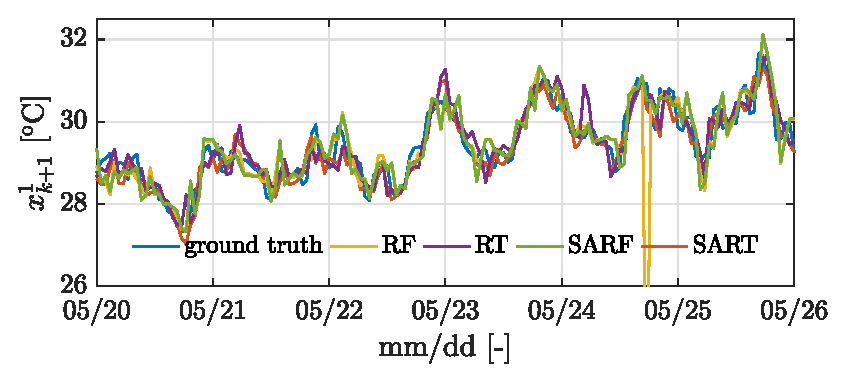
\includegraphics[width=24pc]{figures/validation-s1.eps}
%	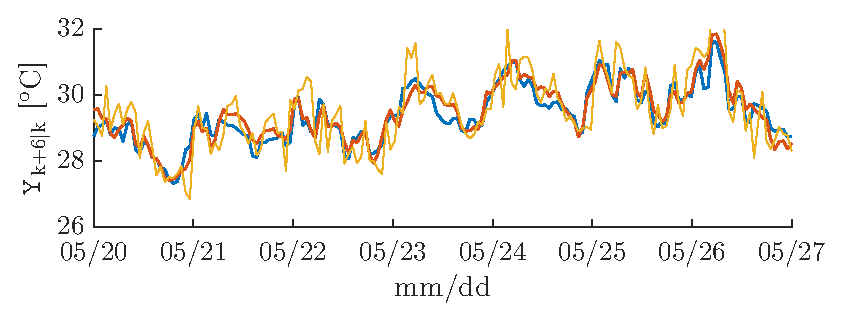
\includegraphics[width=24pc]{figures/validation-s6.eps}
%	\caption{Temperature predictions from a tree and a forest for first step prediction (top) and the 6-hour ahead prediction (bottom). Ensemble method shows a relatively higher accuracy.}
%%	\captionsetup{justification=centering}
%	\label{F:validation}
%\end{figure}

\textbf{Closed-loop simulations.} We simulated the data-driven Switched Affine MPC Problem \ref{pbMPC-SA}, with both model \eqref{eqExtendedSwitchedSystem} (SAMPC-RT) and model \eqref{eqExtendedSwitchedSystemRF} (SAMPC-RF), and DPC Problem \ref{pbDPC}, with both model \eqref{eqAffineModel} (DPC-RT) and model \eqref{eqAffineModelRF} (DPC-RF) using the same cost function and constraints of Problem \ref{pbMPC}. 
We compare the results against the MPC benchmark setup in Problem \ref{pbMPC}.
The results are shown in Fig. \ref{figComparison}. 
The performance is compared for 3 days in winter, i.e. January 28-31 and 3 days in summer, i.e. May 1-3.
The sampling time in the simulations is 1 hour. The control horizon $N$ is 6 hours.
The cooling usage factor $\mathsf{C}$ is constrained in $[0,1]$, the heat input in $[0,23]\ \mathrm{W/m^2}$, and the room temperature in $[19,25]\ \mathrm{^oC}$ during the winter and $[20,26]\ \mathrm{^oC}$ during the summer.
The optimization is solved in MATLAB using CPLEX.
The external disturbances are shown in Figure~\ref{F:dist}.
The reference temperature is chosen to be 22 $\mathrm{^oC}$.
Due to cold weather, which is evident from the dry-bulb temperature, the heating system is switched on during the night to maintain the thermal comfort requirements. When the building is occupied during the day, due to excessive internal gain, the building requires cooling.
The optimal cooling usage factor and the radiator power are shown in Figure~\ref{F:control1} and Figure~\ref{F:control2}.
We can see that Random Forests model based controllers provide inputs that are closer to the optimum and with less peaks.
The optimized cost function is instead shown in Figure~\ref{F:obj}. Results show that the SAMPC-RF is the closest to the optimum, outperforming all the other methods. SAMPC-RT also behave better than its counterpart in DPC, but provides worse performace than DPC-RF due to the high variance problem regression trees are subject to.
For the same reason, that brings to model inaccuracy, the cost for regression trees model based controllers blows up as one of the slack variables is non-zero. The cumulative cost goes extremely high since the parameter $\lambda$ that weights bounds violation is setup to $10^3$.
The room temperature profile is shown in Figure~\ref{F:state}. We can see also here that random forests based controllers provide less spiked trajectories that are closer to the optimum with respect to regression trees based controllers.


\begin{figure}[t!]
	\begin{center}
%		\vspace{1.1cm}
		\subfigure[External disturbances.]{
			\label{F:dist}
			\centering
			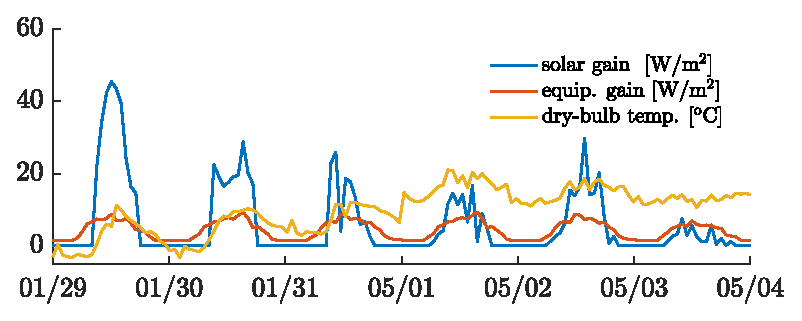
\includegraphics[width=20pc]{figures/disturbances.eps}
		}		
		\subfigure[Optimal control input: cooling usage factor. Random forests-based approaches are closer to MPC.]{
			\label{F:control1}
			\centering
			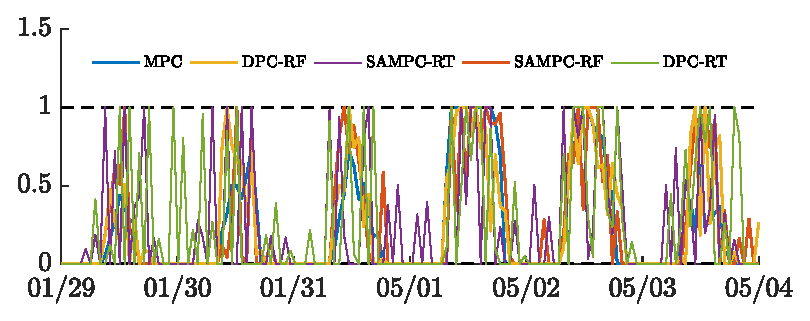
\includegraphics[width=20pc]{figures/cooling.eps}
		}		
		\subfigure[Optimal control input: radiator heat. Random forests-based approaches are closer to MPC.]{
			\label{F:control2}
			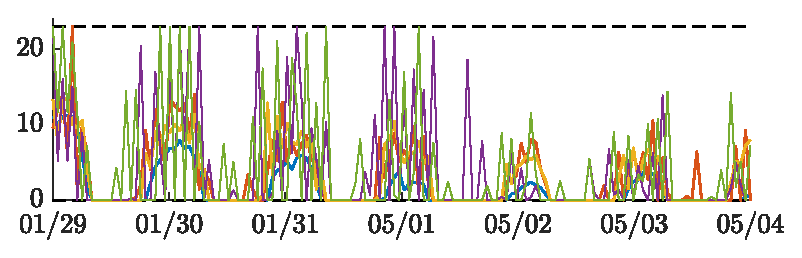
\includegraphics[width=20pc]{figures/heat.eps}
		}		
		\subfigure[Room temperature. Random forests-based approaches track the reference temperature better than regression trees-based ones and provide smoother behaviour.]{
			\label{F:state}
			\centering
			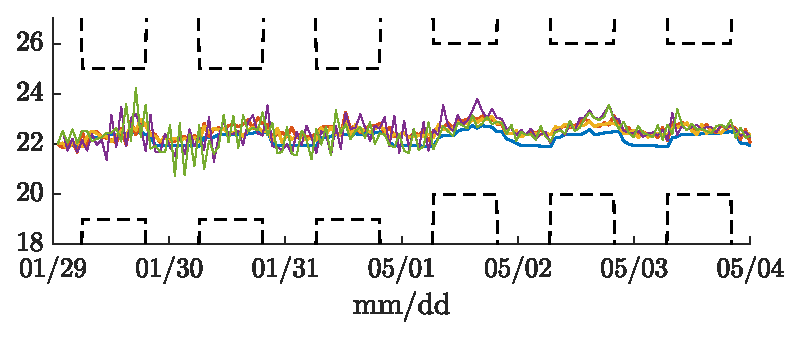
\includegraphics[width=20pc]{figures/temperatures.eps}
		}		
		\subfigure[Cumulative optimal cost after solving optimization. SAMPC-RF shows best performance after the MPC.]{
			\label{F:obj}
			\centering
			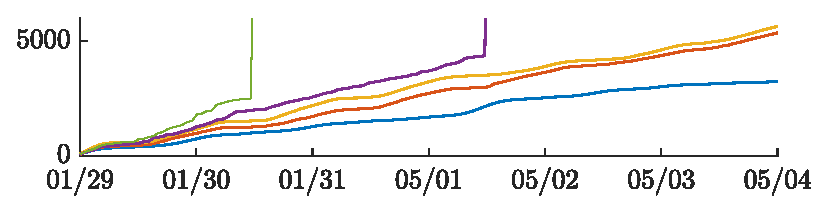
\includegraphics[width=20pc]{figures/cost.eps}
		}
	\end{center}
	\caption{Comparison of optimal performance for 3 days in January and 3 days in May.}
	\label{figComparison}
%	\captionsetup{justification=centering}
\end{figure}


%==============================================================================================================
%==============================================================================================================

\section{CONCLUSIONS AND FUTURE WORK}\label{secConclusion}

In this paper, we provide a methodology to construct a data-driven state-space switched affine model of a system using regression trees and random forests using only historical data.
We setup an MPC problem and compare the performance of our our against another MPC controller, designed using the actual physics-based model, and against DPC controller, that uses static data-driven models.
We compare the results of the approaches on a building energy management problem.
We show that our strategy, without using any physical model of the system, is comparable in terms of optimal cost minimization to MPC which requires a physics-based model, thus bypassing the need for expensive physical modeling in the complex systems like buildings. 
This new approach for data-driven state-space switched affine model is also better than our previous work on control with regression trees and random forests that uses static models.
This work is a staring point for the following future directions.
Future work is focused on applying the proposed methodology on a more complex and realistic EnergyPlus model, for which building a model predictive controller is time and cost prohibitive.
This is because we would need to model intricate details like the geometry and construction layouts, the equipment design and layout plans, material properties, operational schedules etc..
We want also to consider problems where stability is important, i.e. frequency control in a microgrid, and address the problem of providing guarantees on the system and on system properties.
Another direction is to use this approach to improve an existing modeling for which we have partial knowledge of the model by correcting the error approximation using data.

\tiny
\bibliographystyle{ifacconf}
\bibliography{BAS}


\end{document}
